%!TEX root = ./main.tex

In this section we attempt to gain a better understanding of some of the strange behaviour observed in figures \ref{fig:chern_bott_example}-\ref{fig:chern_bott_split_open}. This will be first illustrated by looking at how the Bott index behaves in a system with strip geometry. From this we will see that unusual edge behaviour occurs when a state crosses the Fermi energy, as the edge states do in fig. \ref{fig:strip_energy}.  We then give a qualitative but more general argument to understand the flaws in the Bott index. Finally we briefly discuss the technique of adiabatic flux insertion and its potential for building a more stable definition of the Bott index.

\subsection{Bott Index in Strip Geometry}
As shown in \textsection\ref{sec:QWZ_strip_geometry}, eigenstates in such a system have the form
\begin{align}
    \ket{\psi} = \ket{k_y}\otimes \ket{v_{k_y}^{n,l}},
\end{align}
where $n \in \{ 0,1\}$ tells us which band the state belongs to and $l \in \{ 0,...,L_x\}$ labels each state in that band. We start by restating the expression for Bott index
\begin{align}
    B(\bf A) = -\frac{N}{2\pi} \sum_\alpha \Im \bra{\bf A \alpha} \log \left [ \hat U\hat V\hat U^\dag \hat V^\dag + \hat Q \right ]\ket{ \bf A \alpha},
\end{align}
with
\begin{align}
	\hat U  = \hat P e^{i \delta_x \hat x} \hat P, \ \hat V  = \hat P e^{i \delta_y \hat y} \hat P.
\end{align}
Now we can write $\hat P$ and $\hat Q$ in terms of the semi-Bloch states
\begin{align}
	\hat P &=  \sum_{k_y, l} \ket{k_y} \bra{k_y} \otimes \ket{v_{k_y}^{0,l}}\bra{v_{k_y}^{0,l}} \\ 
	\hat Q  &=  \sum_{k_y, l} \ket{k_y} \bra{k_y} \otimes \ket{v_{k_y}^{1,l}}\bra{v_{k_y}^{1,l}}.
\end{align}
We introduce the reduced projector $\hat P_{k_y}$ and $\hat Q_{k_y}$ as
\begin{align}
	\hat P_{k_y} =  \sum_{l} \ket{v_{k_y}^{0,l}}\bra{v_{k_y}^{0,l}}, \ \hat Q_{k_y} =  \sum_{l} \ket{v_{k_y}^{1,l}}\bra{v_{k_y}^{1,l}}. 
\end{align}
This allows us to re-express $\hat U$ and $\hat V$ as
\begin{align}
	\hat U &= \sum_{k_y} \ket{k_y} \bra{k_y} \otimes \hat P_{k_y}  e^{i \delta_x \hat x}  \hat P_{k_y}  \\ 
	\hat V &=  \sum_{k_y} \ket{k_y} \bra{k_y - \delta_y} \otimes \hat P_{k_y} \hat P_{k_y - \delta_y},
\end{align}
where in the second expression we have used that fact that $  e^{i \delta_y \hat y}\ket{k_y} = \ket{ k_y +  \delta_y}$. Putting this together, we arrive at an expression for the form of $\hat U\hat V\hat U^\dag \hat V^\dag$,
\begin{align}
	\hat U\hat V\hat U^\dag \hat V^\dag = \sum_{k_y} \ket{k_y} \bra{k_y} \otimes \hat P_{k_y}  e^{i \delta_x \hat x}  \hat P_{k_y} \hat P_{k_y - \delta_y} e^{i \delta_x \hat x}  \hat P_{k_y - \delta_y} \hat P_{k_y} .
\end{align}
Now we can add in the rest of the expression for Bott index, arriving at
\begin{align} \label{eqn:strip_bott_index}
	B( A_x ) =  -\frac{L_x}{2\pi} \sum_{k_y , \alpha}  \Im \bra{ A_x , \alpha} \log \left (
	\hat P_{k_y}  e^{i \delta_x \hat x}  \hat P_{k_y} \hat P_{k_y - \delta_y} e^{-i \delta_x \hat x}  \hat P_{k_y - \delta_y} \hat P_{k_y} + \hat Q_{k_y}
	 \right ) \ket{A_x , \alpha},
\end{align}
where we used the expression fact that $|\braket{A_y | k_y }|^2 = \frac{1}{L_y}$ to remove the $k_y$ states. 

\subsubsection{Taylor Expanding the Bott Index}
We can now look at Taylor expanding this expression in $\delta_x$ and $\delta_y$. This calculation has some problems that we will overlook here, but discuss in more detail in \textsection\ref{sec:discontinuities_example}. Our starting point is the operator inside the log in eqn. \ref{eqn:strip_bott_index}, that we will call $\hat M_{k_y}$
\begin{align}
	\hat M_{k_y} &= \hat P_{k_y}  e^{i \delta_x \hat x}  \hat P_{k_y} \hat P_{k_y - \delta_y} e^{-i \delta_x \hat x}  \hat P_{k_y - \delta_y} \hat P_{k_y} + \hat Q_{k_y}.
\end{align}
We now want to Taylor expand this to second order in $\delta_x$ and $\delta_y$. The details of this calculation can be found in Appendix \ref{sec:bott_derivatives}, so we will only quote the result here
\begin{align}
	\hat M_{k_y}  = \1 +i \delta_x \delta_y \hat P_{k_y} \partial_{k_y} \hat X_{k_y} \hat P_{k_y} + O(\delta^3),
\end{align}
where $\hat X_{k_y} = \hat P_{k_y} \hat x  \hat P_{k_y} $ is the projected $x$-operator. Note that in order to get to this expression we have made the assumption that $\hat P_{k_y}$ varies smoothly with $k_y$. This is where the problems will appear, since this assumption is not always valid! Furthermore, this expression will run into trouble in periodic systems, since the $\hat X$ operator is not well-defined in that context. \par
Now, substituting this expression into the Bott index, we get
\begin{align} \label{eqn:ryan_bott_expression}
	B( A_x ) =  -\delta_y\sum_{k_y , \alpha}  \bra{ A_x , \alpha} \left (
	\hat P_{k_y} \partial_{k_y} \hat X_{k_y} \hat P_{k_y}
	 \right ) \ket{A_x , \alpha}
\end{align}
 

\subsubsection{Discontinuities and Null Eigenvalues} \label{sec:discontinuities_example}
In order to figure out what is wrong with the Bott index, we first look at how the $\hat P_{k_y}$ projectors depend on $k_y$. We work in the limit of a large system, allowing us to make the assumption that the edge states are well-separated, being unable to couple to one another, and so must cross the Fermi energy. In open boundary conditions the system has two edge states that cross the Fermi energy (at $E = 0$) at $k_y = \pi$, as seen in figure \ref{fig:strip_energy}\footnote{Actually this is only for $u>0$, if $u<0$ the crossing happens at $k_y = 0$. All of our arguments are identical in both cases so we will ignore this detail and just look at the $u>0$ case.}. These edge states are only present for values of $k_y$ that satisfy
\begin{align}
	-1 < u+\cos k_y < 1.
\end{align}
From this we can extract a value for $k_{min}$ and $k_{max}$, between which the edge states are present. Thus our projector has four different regions depending on the value of $k_y$
\begin{center}
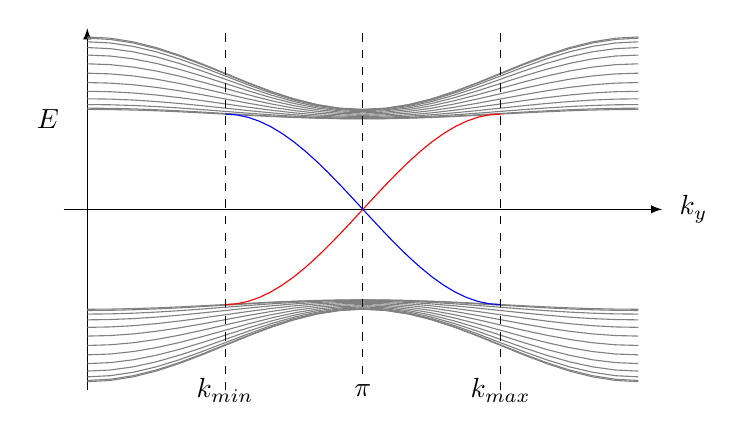
\begin{tikzpicture}

\def \vsize{2.3}
\def \hsize{7}
\def \u{1.3}

\draw [-latex] (0,-\vsize) -- (0,\vsize);
\draw [-latex] (-0.3cm,0) -- (\hsize+0.3,0);

\draw node at (-0.5cm,0.5*\vsize) {$E$};
\draw node at (\hsize cm + 0.7cm, 0) {$k_y$};

\def\bandsteps{12}

\foreach \n in {0, ...,\bandsteps }
{	
	\draw [domain = 0:\hsize, variable= \x, gray] plot ({\x cm},{ 1.1+0.1*(sin(\x*360/\hsize)*sin(\x*360/\hsize) + sin(\n*180/\bandsteps)*sin(\n*180/\bandsteps) + (\u + cos(\x*360/\hsize)  +cos(\n*180/\bandsteps) )*(\u + cos(\x*360/\hsize)  +cos(\n*180/\bandsteps) )  ) });
	\draw [domain = 0:\hsize, variable= \x, gray] plot ({\x cm},{ -1.1-0.1*(sin(\x*360/\hsize)*sin(\x*360/\hsize) + sin(\n*180/\bandsteps)*sin(\n*180/\bandsteps) + (\u + cos(\x*360/\hsize)  +cos(\n*180/\bandsteps) )*(\u + cos(\x*360/\hsize)  +cos(\n*180/\bandsteps) )  ) });
}

\def\scale{1.21}
\draw [domain = -0.25*\hsize:0.25*\hsize, variable= \x, red] plot ({\x +0.5*\hsize},{ \scale*sin(\x*360/\hsize) });
\draw [domain = -0.25*\hsize:0.25*\hsize, variable= \x, blue] plot ({\x +0.5*\hsize},{ -\scale*sin(\x*360/\hsize) });

\draw [dashed] (0.25*\hsize,-\vsize) -- (0.25*\hsize,\vsize);
\draw [dashed] (0.75*\hsize,-\vsize) -- (0.75*\hsize,\vsize);
\draw [dashed] (0.5*\hsize,-\vsize) -- (0.5*\hsize,\vsize);
\draw node [] at (0.25*\hsize,-\vsize) {$k_{min}$};
\draw node [] at (0.75*\hsize,-\vsize) {$k_{max}$};
\draw node [fill=white] at (0.5*\hsize,-\vsize) {$\pi$};
\end{tikzpicture}
\end{center}
\begin{center}
\begin{tabular}{ r l }
 $k_y \in (0, k_{min})$ : & $P_{k_y}$ contains $L_x$ bulk states \\ 
 $k_y \in (k_{min},\pi)$ : & $P_{k_y}$ contains $L_x -1 $ bulk states and one right-edge state  \\  
  $k_y =\pi $ : & $P_{k_y}$ contains $L_x -1 $ bulk states and both edge states  \\  
 $k_y \in (\pi, k_{max})$ : & $P_{k_y}$ contains $L_x -1 $ bulk states and one left-edge state  \\ 
 $k_y \in ( k_{max} , 2\pi)$ : & $P_{k_y}$ contains $L_x$ bulk states
\end{tabular}
\end{center}
At $k_{min}$ and $k_{max}$, a bulk state smoothly transitions into an edge state and vice-versa, so the change in $P_{k_y}$ is continuous. However at $k_y = \pi$, a right-edge state vanishes and a left-edge state appears, causing $P_{k_y}$ to change discontinuously. These states are able to suddenly disappear and appear because they cross the Fermi level, which is assumed to be a hard cutoff. As we will see, this discontinuity is the source of all of our troubles.\par
To understand where this causes problems we will expand the expression in eqn. \ref{eqn:strip_bott_index} to first order in $\delta_x$. This is reasonable since we are already working under the assumption that $L_x$ is large. We look only at the operator that appears in the logarithm, which we label $\hat M_{k_y}$,
\begin{align}
	\hat M_{k_y} &= \hat P_{k_y}  e^{i \delta_x \hat x}  \hat P_{k_y} \hat P_{k_y - \delta_y} e^{-i \delta_x \hat x}  \hat P_{k_y - \delta_y} \hat P_{k_y} + \hat Q_{k_y} \\
	\begin{split}\label{eqn:m_taylor}
		& = \hat P_{k_y} \hat P_{k_y - \delta_y} \hat P_{k_y} + \hat Q_{k_y} \\
		&\phantom{=}\, + i \delta_x \hat P_{k_y} \left ( \hat X_{k_y} - \hat X_{k_y- \delta_y }  \right )\hat P_{k_y - \delta_y} \hat P_{k_y}
	+ O(\delta_x^2).
	\end{split}
\end{align}
Now suppose that we are looking at a particular value of $k_y$ such that $k_y - \delta_y < \pi < k_y$, furthermore we will assume that  $\delta_y$ is extremely small, ensuring that the energy eigenstates themselves do not change significantly between $k_y - \delta_y $ and $ k_y$. This means that $P_{k_y}$ contains a left-edge state and $P_{k_y-\delta_y}$ contains a right-edge state. Thus the operator $\hat P_{k_y} \hat P_{k_y - \delta_y} \hat P_{k_y}$ only contains bulk states\footnote{This is not quite true, the states themselves change slightly with $k_y$, so this statement is approximate rather than exact. However as the value of $\delta_y$ gets smaller this statement gets closer and closer to being exact.}. $\hat Q_{k_y}$ will only contain a right-edge state, so the combination $ \hat P_{k_y} \hat P_{k_y - \delta_y} \hat P_{k_y} + \hat Q_{k_y} $ looks like the identity but with a single missing eigenvalue -- where the missing left-edge state is. This will occur whenever $k_y$ and $k_y - \delta_y$ sit on opposite sides of a point where the edge states cross the Fermi level.\par
This causes problems in our calculations. As we see in expression \ref{eqn:m_taylor}, $\hat M_{k_y}$ looks like it should have the form $\hat M_{k_y} = \1 + W_{\textup{small}}$, where $W$ is just some operator with eigenvalues $\ll 1$. This would mean that $\log \hat M_{k_y} \approx W_{\textup{small}}$.  However for certain values of $k_y$, the the operator $ \hat P_{k_y} \hat P_{k_y - \delta_y} \hat P_{k_y} + \hat Q_{k_y}$ is almost the identity but with one very small eigenvalue. When we take a log of the operator, this missing eigenvalue gives a huge contribution, since the log diverges at zero. \par
Now we can see where the strange edge behaviour of the Bott index comes from. This tiny eigenvalue of $\hat M_{k_y}$ has as its eigenvector the missing state from $ \hat P_{k_y} \hat P_{k_y - \delta_y} \hat P_{k_y} + \hat Q_{k_y} $. This missing state is always an edge state, so effect is to create a large distortion to the Bott index that lives on the support of that edge state. This is precisely what we see when we calculate the Bott index in strip geometry, as shown in fig. \ref{fig:edge_bott}.
\begin{figure}[t]
\begin{center}
 \includegraphics[width=0.8\textwidth]{edge_bott}
\caption{Strip Bott index calculated for a material with $L_x  = L_y = 70$, $u = 1.4$ compared to the probability distribution of the right edge state. A large discontinuity can be seen on the right hand side of the Bott index that closely matches the shape of the right edge state, supporting our assertion that the edge behaviour of the Bott index is due to a term in the sum that lives on the support of one edge state.}
\label{fig:edge_bott}
\end{center}
\end{figure}

\subsubsection{Generalising the Argument}
We can now give a looser and more general understanding for why these problems are appearing in our calculations. When we calculate the Chern number of a band, what we essentially want to do is take every state in that band, and push it adiabatically around a plaquette in $k$-space. We look at the phase that each state accumulates, and sum them to get $\mathcal Q$.

\begin{center}
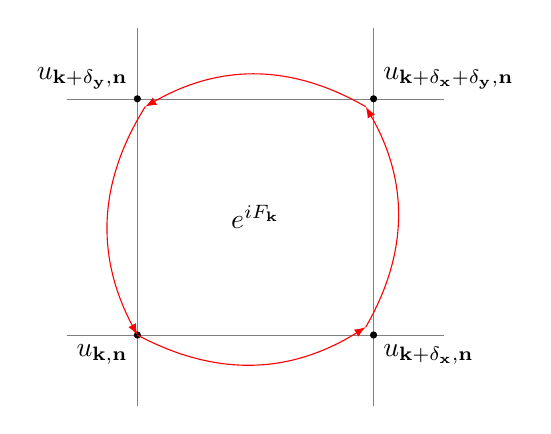
\begin{tikzpicture}

\def \gridsize{3}
\def \in {0.4}
\def\lineoffset{0.1}

\draw[step=\gridsize cm, help lines] (-0.3*\gridsize,-0.3*\gridsize) grid (1.3*\gridsize,1.3*\gridsize);

 
\foreach \x in {0, ..., 1}{
\foreach \y in {0, ..., 1}{
\fill[] (\x*\gridsize , \y*\gridsize) circle (1.3pt);
}}

\draw [red , -latex] (0,0) to [bend right] (\gridsize-\lineoffset,0+\lineoffset);
\draw [red , -latex] (\gridsize-\lineoffset,0+\lineoffset) to [bend right] (\gridsize-\lineoffset,\gridsize-\lineoffset);
\draw [red , -latex] (\gridsize-\lineoffset,\gridsize-\lineoffset) to [bend right] (0+\lineoffset,\gridsize-\lineoffset);
\draw [red , -latex] (0+\lineoffset,\gridsize-\lineoffset) to [bend right] (0,0);



 \draw node [fill= white] at ( 0.5*\gridsize, 0.5*\gridsize) {$e^{iF_{\bf k}}$};

\draw node [below left] at (0,0) {$\ket{u_{\bf k, n}}$};
\draw node [below right] at (\gridsize,0) {$\ket{u_{\bf k + \bm \delta_x, n}}$};
\draw node [above right] at (\gridsize,\gridsize) {$\ket{u_{\bf k + \bm \delta_x + \bm \delta_y , n}}$};
\draw node [above left] at (0,+\gridsize) {$\ket{u_{\bf k + \bm \delta_y, n}}$};

\end{tikzpicture}
\end{center}


However, this is not quite what happens when we calculate the Bott index! When we find the Bott index, what we are doing is using the $e^{i\delta_x \hat x}$ and $e^{i\delta_y \hat y}$ operators to shift the $\ket k$ part of each energy eigenstate, allowing us to take an inner product of adjacent states in $k$-space. We are looking at eigenstates that are adjacent to one another in $\hat P$ and expecting these to be closely adiabatically connected. When the system has no edge states -- no states cross the Fermi level -- this expectation proves to be correct, so the calculation is equivalent to pushing one state around a loop.
\begin{center}
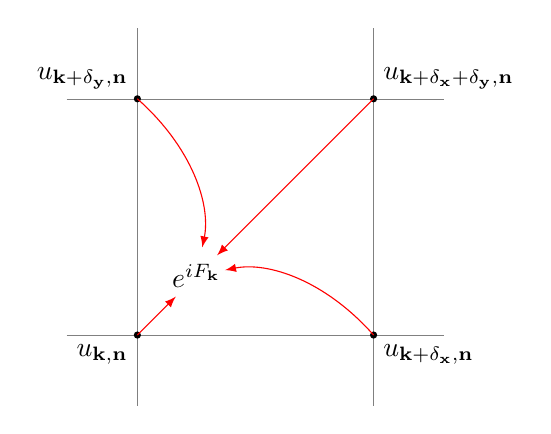
\begin{tikzpicture}

\def \gridsize{3}
\def \in {0.4}
\def\labeloffset{0.5}

\draw[step=\gridsize cm, help lines] (-0.3*\gridsize,-0.3*\gridsize) grid (1.3*\gridsize,1.3*\gridsize);

 
\foreach \x in {0, ..., 1}{
\foreach \y in {0, ..., 1}{
\fill[] (\x*\gridsize , \y*\gridsize) circle (1.3pt);
}}

 \draw node [fill= white] at ( 0.25*\gridsize, 0.25*\gridsize) {$e^{iF_{\bf k}}$};

\draw [red,-latex,shorten >=0.37cm ] (\gridsize,0) to [bend right] (0.25*\gridsize, 0.25*\gridsize);
\draw [red , -latex,shorten >=0.37cm] (\gridsize,\gridsize) to [] (0.25*\gridsize, 0.25*\gridsize);
\draw [red, -latex,shorten >=0.37cm] (0,\gridsize) to [bend left] (0.25*\gridsize, 0.25*\gridsize);
\draw [red, -latex,shorten >=0.37cm] (0,0) to [] (0.25*\gridsize, 0.25*\gridsize);



\draw node [below left] at (0,0) {$\ket{u_{\bf k, n}}$};
\draw node [below right] at (\gridsize,0) {$\ket{u_{\bf k + \bm \delta_x, n}}$};
\draw node [above right] at (\gridsize,\gridsize) {$\ket{u_{\bf k + \bm \delta_x + \bm \delta_y , n}}$};
\draw node [above left] at (0,+\gridsize) {$\ket{u_{\bf k + \bm \delta_y, n}}$};

\end{tikzpicture}
\end{center}
However when a state crosses the Fermi level, this allows the states in $\hat P$ to change discontinuously as you try to translate $\hat P$ in $k$-space. That means when you are comparing states that are adjacent to one another, you end up inadvertently comparing states on either side of some discontinuous jump in $\hat P$. This is exactly what happened in \textsection\ref{sec:discontinuities_example}, where we ended up trying to take a product between a left edge state and a right edge state. Since these states are not closely related to one another, we cannot expect to get a reasonable number for the relative phase between them, and our calculation breaks down.\par
Now that we have a sense of what is going wrong, we can try to construct a definition of the Bott index that does not suffer from these issues. Central to this will be the idea of trying to build a Bott index using operators that translate us adiabatically through $k$-space.

\subsection{Adiabatic Bott Index}

We now try and invent something that looks like a Bott index, but relies only on adiabatic translations through $k$-space, as hopefully this will allow us to avoid hitting discontinuities in our projector. This work is unfinished, here we will lay some of the groundwork and explain the central idea, however it is currently unclear whether this method will produce the desired result. Central to this is the notion of adiabatic flux insertion, a technique that has been used to understand fractionalisation in quantum many body systems \cite{oshikawa_fractionalization_2006}. We start by looking at how to include the presence of a magnetic field in a lattice system -- using Peierls substitution. We can then use this to construct a set of operators representing the slow insertion of magnetic flux through our system. Hopefully these should provide a pathway to constructing $k$-translation operators with which to define a stabilised Bott index.

\subsubsection{Peierls Substitution}

We first introduce an approximate technique to describe the effect of a slowly-varying magnetic field on a tight-binding quantum system first introduced in \cite{peierls_zur_1933}, although a description in English can be found in \cite{hofstadter_energy_1976}. The Peierls substitution states that in the presence of a magnetic vector potential $\bf A$, the translation operators that form the Hamiltonian change according to
\begin{align}
	\hat T_x \rightarrow \ket{\bf m + 1_x}\bra{\bf m} e^{i \theta_{\bf m}^x}, \ \hat T_y \rightarrow \ket{\bf m + 1_y}\bra{\bf m} e^{i \theta_{\bf m}^y},
\end{align}
where $\theta$ is just the line integral of the vector potential between two adjacent sites on the lattice,
\begin{align}
	\theta_{\bf m}^x = \frac{q}{\hbar}\int_{\bf m}^{\bf m + 1_x} \bf A(\bf r) \cdot d\bf r, \ \theta_{\bf m}^y = \frac{q}{\hbar}\int_{\bf m}^{\bf m + 1_y} \bf A(\bf r) \cdot d\bf r.
\end{align}\par
Now suppose that we have some material on a two dimensional square lattice and we introduce a uniform potential $\bf A$ across the whole material. If the lattice points are equally spaced apart, this will mean that every nearest-neighbour translation operator picks up a constant phase $\theta_x$ or $\theta_y$, and each longer-range operator picks up a phase proportional to the distance in each direction. Thus a Hamiltonian in such a system given by
\begin{align}
	\hat H  = \sum_{\bf m, \bf n} \ket{\bf m} \bra{\bf n} \otimes \hat H^{int}_{\bf m, \bf n}
\end{align}
is modified to
\begin{align}
	\hat H(\bf A)  = \sum_{\bf m, \bf n} \ket{\bf m} \bra{\bf n} e^{i \theta_x(m_x - n_x) + \theta_y(m_y - n_y)} \otimes \hat H^{int}_{\bf m, \bf n}.
\end{align}
This is exactly equivalent to making the following transformation
\begin{align}
	\hat H \rightarrow \hat H (\bf A) = e^{i \bm \theta \cdot \hat{ \bf x}} \hat H e^{-i \bm \theta \cdot  \hat{ \bf x}},
\end{align}
so we realise that we have already been working with these kinds of transformations already, and know exactly their effect -- to translate our states around $k$-space by the vector $\bm \theta$!

\begin{shaded}
	Something weird is going on -- for values of $\theta \neq \frac{2\pi p}{L_x}$ where $p$ is an integer, the exponential operator here is not periodic with the system and so isn't well-defined! It turns out this does not matter, since the operator is only used to add a phase to the off-diagonal elements of $\hat H$.
\end{shaded}

\subsubsection{Adiabatic Flux Insertion}

The idea here is that we can use the slow insertion of magnetic flux to transport our states around the Brillouin zone. We define a pair of operators $\hat{\mathcal{F}}_x$ and $\hat{\mathcal{F}}_y$ that represent the gradual ramping up of a magnetic vector potential in either the $x$ or the $y$-direction. This is ramped up from $A = 0$ to 
\begin{align}
	A_x = \frac{2\pi\hbar}{q \Delta_x L_x},
\end{align}
where $\Delta_x$ is the distance between unit cells in the lattice. We use the equivalent expression for $\hat{\mathcal F}_y$. These values are chosen such that at the end $\theta_x = \frac{2\pi}{L_x}$ and $\theta_y = \frac{2\pi}{L_y}$. When acted on a state $\ket{\psi_{\bf k, n}}$, the operator $\hat{\mathcal{F}}_x$ should be able to transform it to $\ket{\psi_{\bf k + \delta_x, n}}$. Since it is adiabatic it will not mix between states  at different energy. Furthermore, the operator is local, and this should ensure that in a large system it is prohibited from mixing between a left edge state and a right edge state.\par
Thus we can use these operators in place of $e^{i \delta_x \hat x}$ and $e^{i \delta_y \hat y}$ in the definition of the Bott index. These have the advantage that when acted on a projector containing bulk states and one left edge state, for example, they will only be able to map it to a new projector containing the same types of states, but translated in $k$-space. This allows us to avoid the discontinuities encountered in \textsection\ref{sec:discontinuities_example}. In the case where there are no states crossing the Fermi level and $\hat P_{k_y}$ is continuous it should be exactly identical to the standard definition of Bott index.

